\section{Evaluation details}
\label{qoala:sec:app:evaluation}

\subsection{Simulator setup}
All simulations have been done with the simulation package found at~\cite{qoala2023simulator}
and were run on a machine using 80 Intel Xeon Gold cores at 3.9 GHz and 192 GB of RAM.

\textbf{Code availability.}
All code used for the evaluations is available in the \texttt{evaluation/} folder~\cite{qoala2023simulator}.
For each evaluation done (each subsection in \cref{qoala:sec:evaluation}, it includes the Qoala program source code, the scripts for running the simulations, the scripts for producing the plots, and a \texttt{README} that explains how to use the code.
In the source code, the term \textit{time bin} is used for what we here call \textit{time slot}.

\subsection{Hardware parameters}
In this section we describe the characteristics of the hardware types that have been used in our evaluations.
For the evaluation in \cref{qoala:sec:demonstrating_architecture_effectiveness} we simulated all three types below;
for the other evaluations we only considered the generic hardware type.

\subsubsection{Generic hardware}
The allowed gate set is expressed as a particular NetQASM flavour~\cite{dahlberg2022netqasm}.

\begin{itemize}
  \item Allowed single-qubit gates (vanilla NetQASM flavour~\cite{dahlberg2022netqasm}):
  \texttt{init}, \texttt{rot\_x}, \texttt{rot\_y}, \texttt{rot\_z}, \texttt{x}, \texttt{y}, \texttt{z}, \texttt{h}, \texttt{meas}.
  \item Allowed two-qubit gates (vanilla NetQASM flavour): \texttt{cnot}, \texttt{cphase}.
\end{itemize}

Qubit decoherence times are expressed as T1 (amplitude damping) and T2 (dephasing time), which is commonly done in quantum computing.
Unless stated otherwise in the evaluation details below, the default noise and duration parameters used for the generic hardware are:
\begin{itemize}
  \item Single-qubit duration: $5 \cdot 10^3$ ns.
  \item Two-qubit duration: $200 \cdot 10^3$ ns.
  \item Qubit T1 time: $10^9$ ns.
  \item Qubit T2 time: $10^8$ ns.
\end{itemize}


\subsubsection{NV hardware}
Values from~\cite{avis2023requirements} and private communication.

\begin{itemize}
  \item Allowed single-qubit gates on communication qubit (NV NetQASM flavour): \texttt{init}, \texttt{rot\_x}, \texttt{rot\_y}, \texttt{meas}.
  \item Allowed single-qubit gates on memory qubit (NV NetQASM flavour): \texttt{init}, \texttt{rot\_x}, \texttt{rot\_y}, \texttt{rot\_z}, \texttt{meas}.
  \item Allowed two-qubit gates between communication qubit and memory qubit (NV NetQASM flavour): \texttt{crot\_x}, \texttt{crot\_y}.
\end{itemize}

Unless stated otherwise in the evaluation details below, the default noise and duration parameters used for the NV hardware are:
\begin{itemize}
  \item Single-qubit duration on communication qubit: 300 ns.
  \item Single-qubit duration on memory qubit: $1.2$ ms.
  \item Two-qubit duration: 1 ms.
  \item Communication qubit T1 time: 3600 ms
  \item Communication qubit T2 time: 500 ms
  \item Memory qubit T1 time: 35000 ms
  \item Memory qubit T2 time: 1 ms
\end{itemize}

\subsubsection{Trapped Ion hardware}
Values from~\cite{avis2023requirements} and private communication.

\begin{itemize}
  \item Allowed single-qubit gates (trapped ion NetQASM flavour): \texttt{init}, \texttt{rot\_z}, \texttt{meas}.
  \item Allowed all-qubit gates (trapped ion NetQASM flavour): \texttt{init\_all}, \texttt{meas\_all}, \texttt{rot\_x\_all}, \texttt{rot\_y\_all}, \texttt{rot\_z\_all}, \texttt{bichromatic}.
\end{itemize}


The effect of applying a bichromatic gate is expressed as
\[
   U_{XX}(\theta) = \exp(-i \frac{\theta}{2} \sum_{i<j} \sigma_X^{(i)} \sigma_X^{(j)})
\]

for some angle $\theta$.

Unless stated otherwise in the evaluation details below, the default noise and duration parameters used for the Trapped Ion hardware are:
\begin{itemize}
  \item Single-qubit duration on communication qubit: 26.6 $\mu s$.
  \item All-qubit duration: 85 ms.
  \item Qubit T1 time: $\infty$.
  \item Qubit T2 time: 85 ms.
\end{itemize}

\subsubsection{NetQASM gate sequence for CNOT on Trapped Ion hardware}
We list the sequence of netqasm instructions to effectively apply a CNOT gates on two qubits, which is non-trivial.

Assuming 2 qubits are in use, CNOT gate between qubit 0 and qubit 1 on trapped ion:
\begin{lstlisting}
  NETQASM:
    // cnot between q0 and q1
    rot_x_all 8 4
    rot_z Q0 8 4
    rot_x_all 24 4
    bichromatic 8 4
    rot_x_all 24 4
    rot_x_all 8 4
    rot_z Q0 24 4
    rot_x_all 24 4
\end{lstlisting}

\begin{table*}[]
\begin{tabular}{|l|l|l|l|l|l|}
\hline
\textbf{Application} & \textbf{\begin{tabular}[c]{@{}l@{}}Number \\ of nodes\end{tabular}} & \textbf{\begin{tabular}[c]{@{}l@{}}Number of\\ EPR pairs\\ per instance\end{tabular}} & \textbf{\begin{tabular}[c]{@{}l@{}}Max number\\ of qubits\\ per node\end{tabular}} & \textbf{\begin{tabular}[c]{@{}l@{}}Number of \\ instances\end{tabular}} & \textbf{\begin{tabular}[c]{@{}l@{}}Simulation\\ duration (s)\end{tabular}} \\ \hline
A1. QKD              & 2   & 1000   & 1     & 1000     & 2166   \\ \hline
A2. BQC              & 2   & 2      & 2     & 1000     & 227    \\ \hline
A3. Teleportation    & 2   & 1      & 2     & 1000     & 24     \\ \hline
A4. Ping-pong        & 2   & 2      & 2     & 1000     & 35     \\ \hline
A5. GHZ              & 3   & 4      & 2     & 1000     & 41     \\ \hline
\end{tabular}
\caption{Overview of application used in the evaluation described in \cref{qoala:sec:demonstrating_architecture_effectiveness}.
Each application was simulated three times, once for each hardware type (generic, NV, Trapped Ion).
Each simulation was for 1000 instances of the application.
The simulation duration is an average over the three simulations per application.
}
\label{tab:app:applications}
\end{table*}


\begin{figure*}
    \centering

    \subfloat[\centering \label{qoala:fig:app:qkd_circuit}]{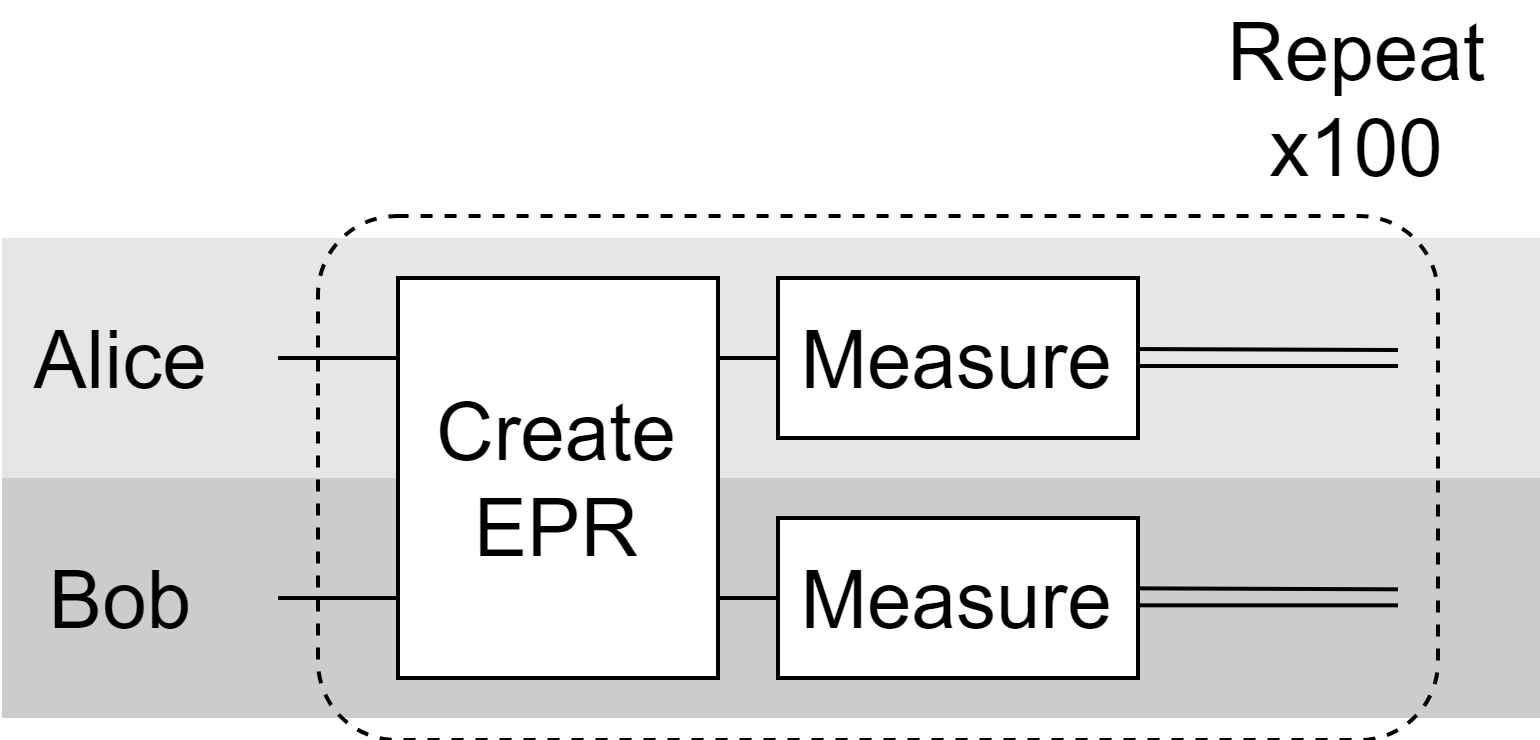
\includegraphics[scale=0.9]{figures/qoala/qkd_circuit.png}}
    \vspace{1cm}
    \subfloat[\centering \label{qoala:fig:app:teleport_circuit}]{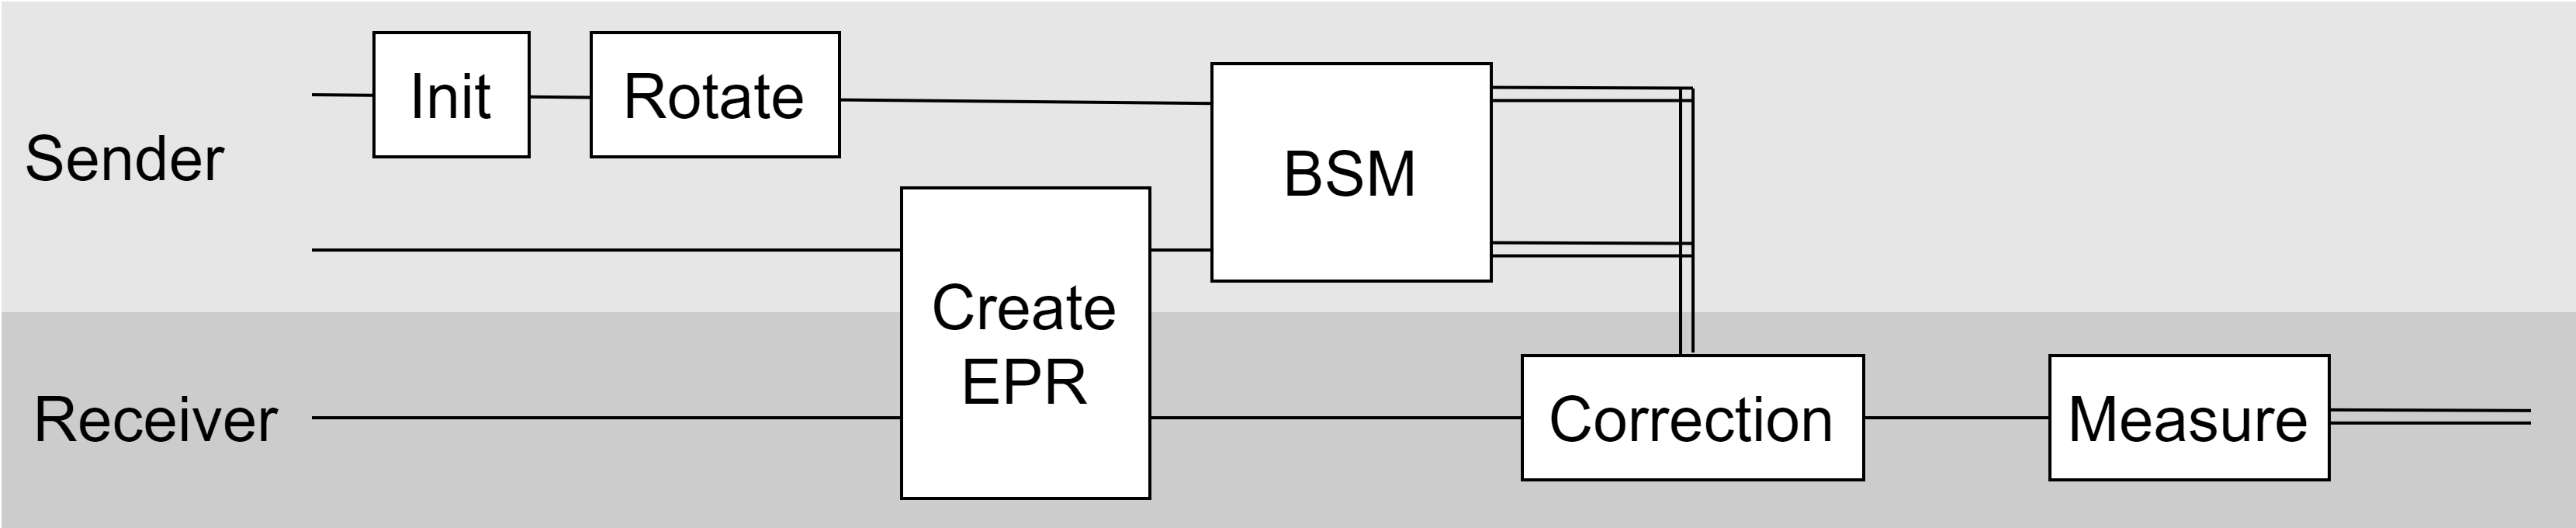
\includegraphics[scale=0.5]{figures/qoala/teleport_circuit.png}}
    \vspace{1cm}
    \subfloat[\centering \label{qoala:fig:app:pingpong_circuit}]{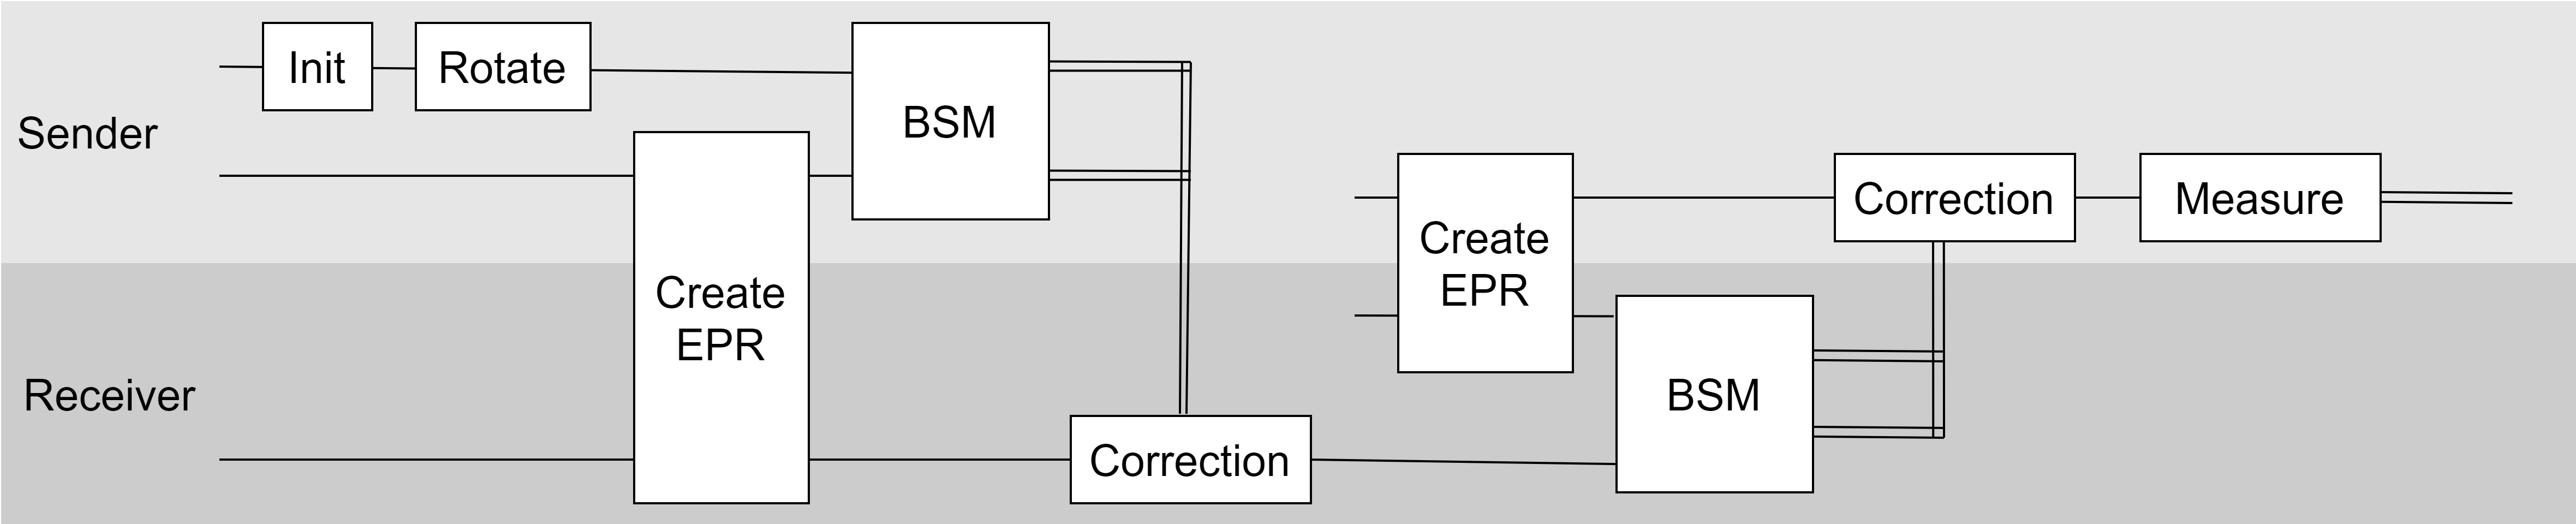
\includegraphics[scale=0.4]{figures/qoala/pingpong_circuit.png}}
    \caption{
    Circuit for applications A1 (QKD), A3 (Teleport) and A4 (ping-pong) from \cref{qoala:sec:evaluation}.
    Single lines represent qubits. Double lines represent classical values.
    (a) QKD (A1). Two nodes repeatedly generate entangled pairs which are immediately measured.
    (b) Teleport (A3). A sender node (having 2 qubits) teleport a state to a receiver node. The sender applies local quantum operations (initialization, qubit rotation gates).
    The sender and receiver create an entangled pair. The sender performs local quantum gates and measurements resulting in classical outcomes.
    The sender sends the classical outcomes to the receiver. Based on the outcomes the receiver applies local quantum gates and measurement.
    (c) Ping-pong (A4). The sender teleports a state to the receiver and the receiver immediately teleports it back to the sender. In total, 2 entangled pairs are created.
    }
    \label{qoala:fig:app:circuits_1}
\end{figure*}

\begin{figure*}
    \centering

    \subfloat[\centering \label{qoala:fig:app:vbqc_circuit}]{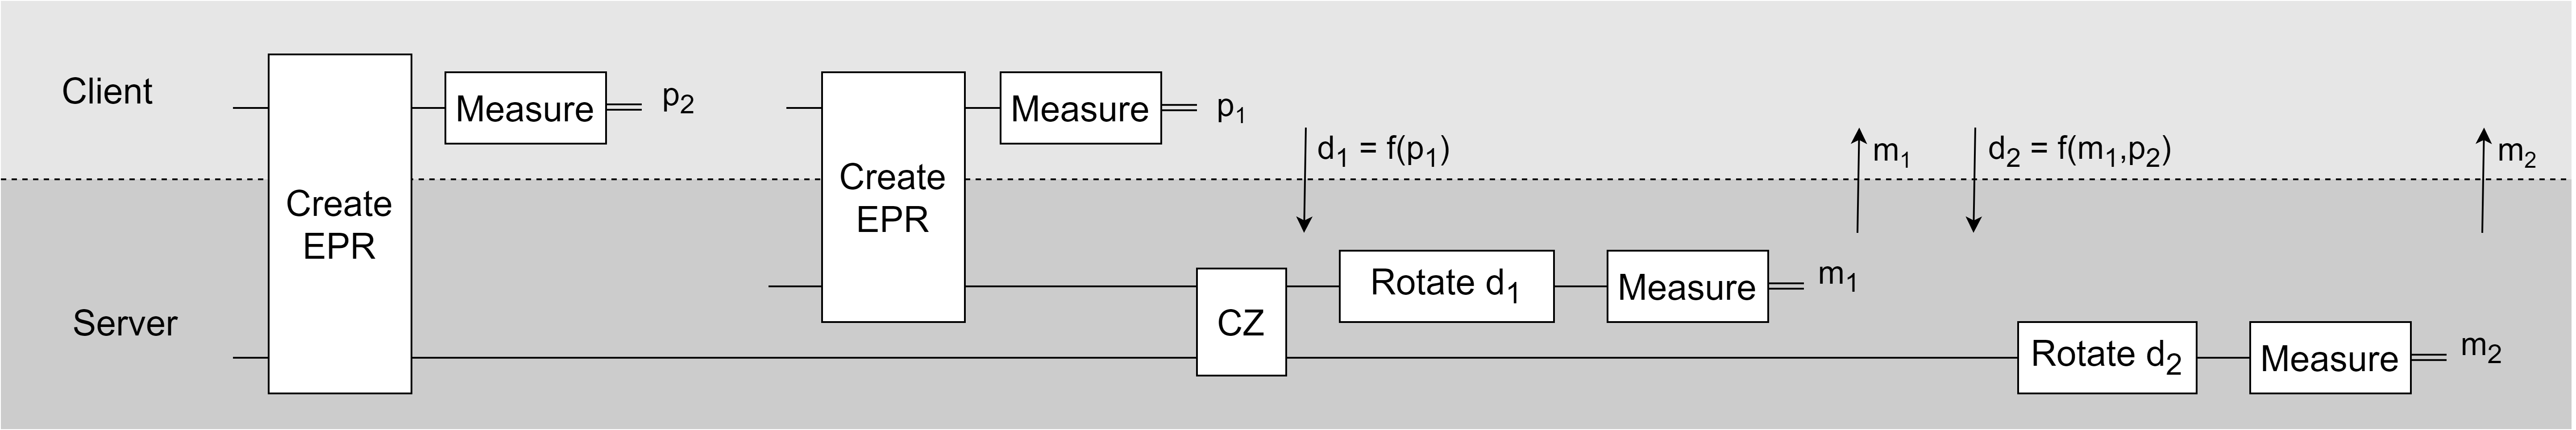
\includegraphics[scale=0.3]{figures/qoala/vbqc_circuit.png}}
    \vspace{1cm}
    \subfloat[\centering \label{qoala:fig:app:ghz_circuit}]{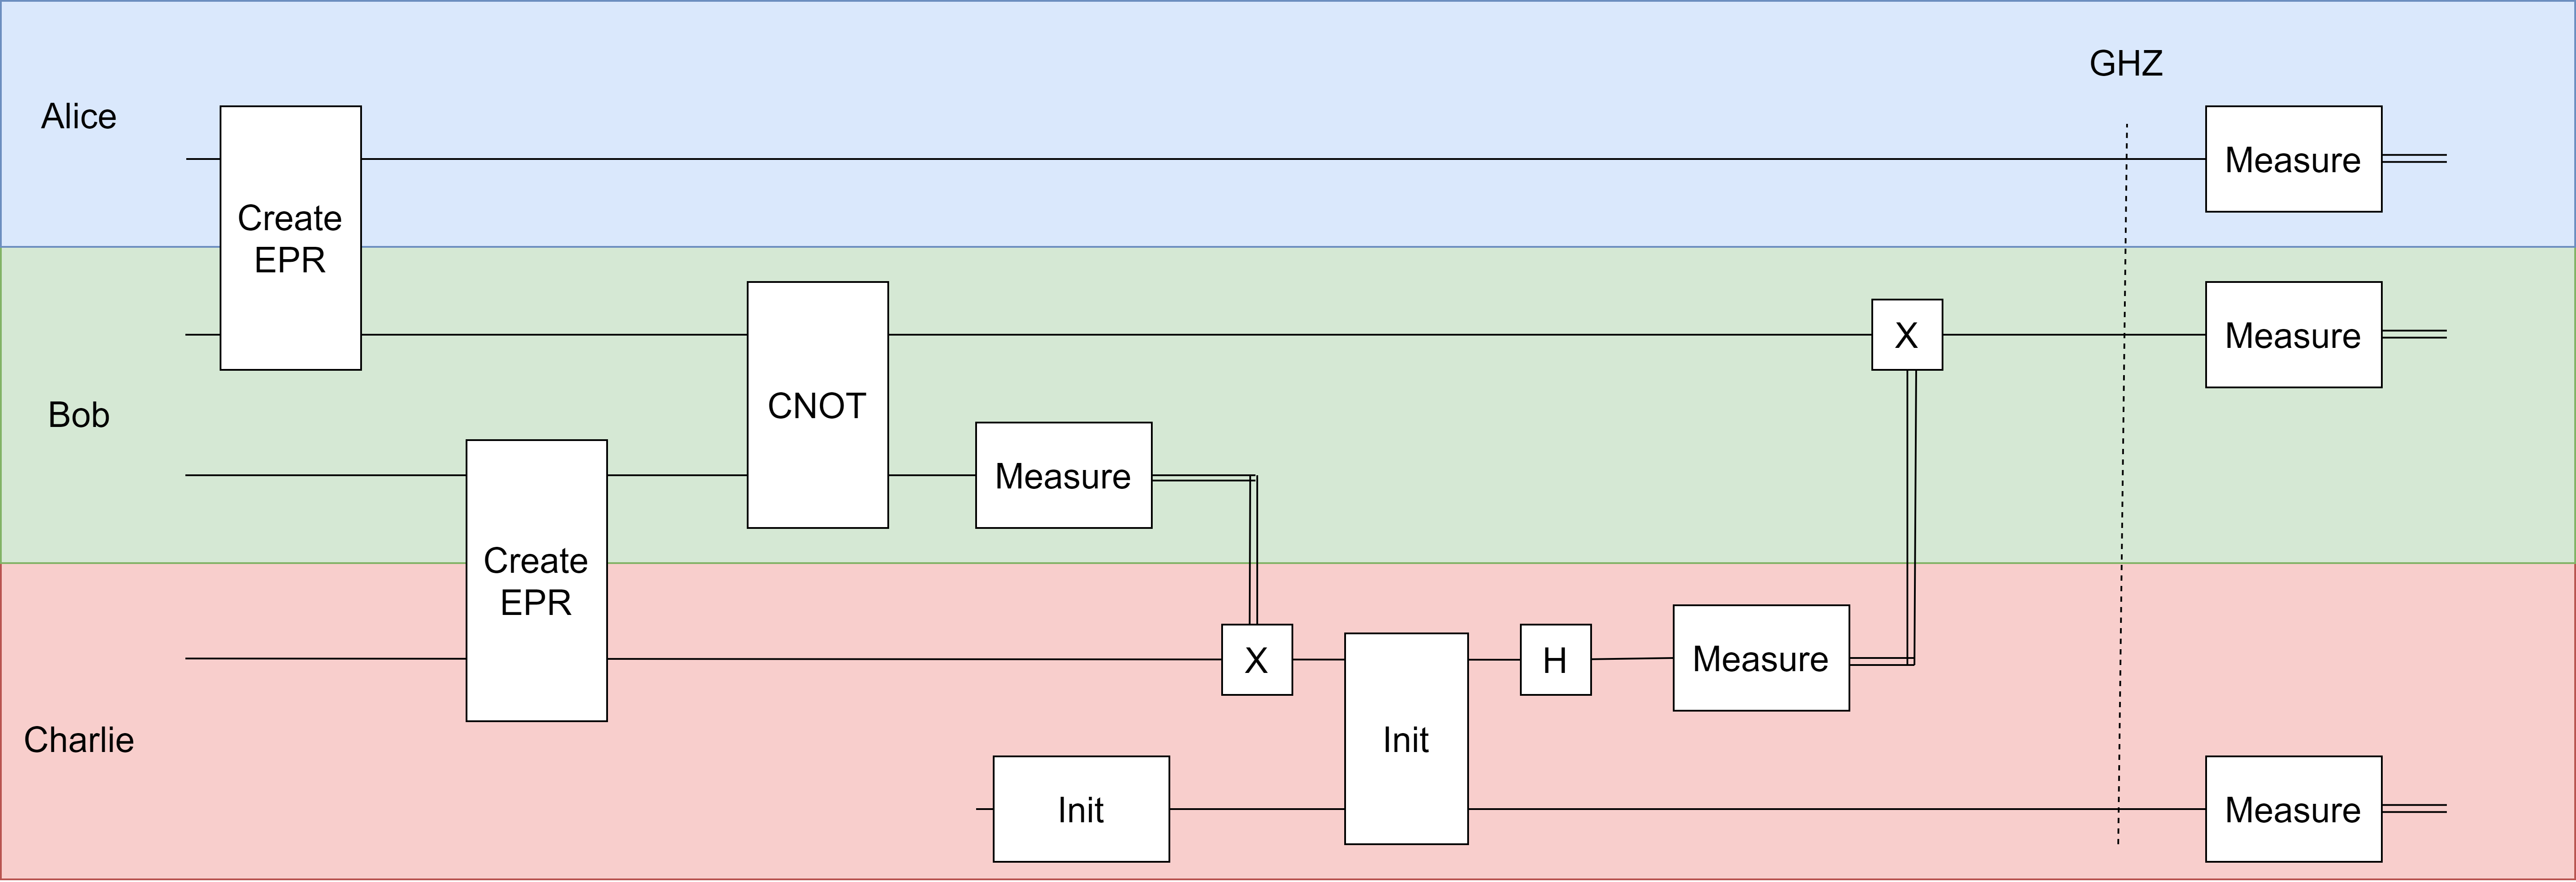
\includegraphics[scale=0.3]{figures/qoala/ghz_circuit.png}}
    \vspace{1cm}

    \caption{
    Circuit for applications A2 (BQC) and A5 (GHZ) from \cref{qoala:sec:evaluation}.
    Single lines represent qubits. Double lines represent classical values.
    (a) BQC (A2). A client node remotely prepares two qubits on a server node by creating an entangled pair and locally measuring its qubits, resulting in classical outcomes $p_1$ and $p_2$.
    The server applies a local two-qubit gate (CZ or cphase) on its qubits.
    The client sends a classical value $d_1$ which it calculates based on $p_1$ and other application input values.
    The server applies local gates based on $d_1$ and measures, resulting in classical value $m_1$ which it sends to the client.
    The client sends a classical value $d_2$ which it calculates based on $p_2$, $m_1$ and other application input values.
    The server applies local gates based on $d_2$ and measures, resulting in classical value $m_2$ which it sends to the client.
    The client uses the values $m_2$ to calculate the final result (not in the Figure).
    (b) Three nodes (Alice, Bob, and Charlie) create pair-wise entangled pairs. Bob applies local gates and measures one of his qubits, sending the outcomes to Charlie.
    Based on this outcome, Charlie performs local operations and sends a measurement outcome back to Bob.
    At the time of the vertical dashed line, the three nodes share a 3-qubit GHZ state. They all measure and check their correlations.
    }
    \label{qoala:fig:app:circuits_2}
\end{figure*}



\subsection{Details for: Demonstrating the architecture's effectiveness}
\label{qoala:sec:app:details_6_1}
A free network schedule was used, meaning that there were no specific time slots, and entanglement generation was allowed at any time.
Such a free network schedule was justified since we considered only whether the application ran successfully

All applications were run with both (a) hardware-validated parameters (see above); all executions were successful and (b) no-noise versions of these parameters (same durations of all operations but no decoherence nor gate noise); these were used to check if the expected outcomes were obtained.

\Cref{tab:app:applications} provides an overview of the applications.

\textbf{Quantum Key Distribution (QKD)}. 
Two programs (on two nodes): Alice and Bob. $N$ EPR are pairs are generated. Each generated pair is immediately measured by both programs.
This results in both programs having $N$ classical outcome bits.
See \cref{qoala:fig:app:qkd_circuit} for the circuit.
Success per instance is determined by checking that Alice and Bob got the same $N$ outcomes bits.
For the evaluation, we ran 1000 instances, each creating 1000 EPR pairs.

\textbf{Teleportation}.
Two programs (on two nodes): Sender and Receiver. The Sender teleports a \textit{state} (which is state is an argument to the Sender program) to the Receiver.
The Receiver measures in a \textit{basis} (which basis is an argument to the Receiver program) and obtains a single classical outcome bit which is the result of the application.
See \cref{qoala:fig:app:teleport_circuit} for the circuit.
Success per instance is determined by checking that the Receiver got the expected outcome bit (which depends on the combination of state and basis).
For the evaluation, we ran 1000 instances.

For each of the Sender program instances, the \textit{state} argument was chosen evenly from the following:
$\ket{0}$,
$\ket{1}$,
$\ket{+} = 1/\sqrt{2} (\ket{0} + \ket{1})$,
$\ket{-} = 1/\sqrt{2} (\ket{0} - \ket{1})$,
$\ket{+i} = 1/\sqrt{2} (\ket{0} + i \ket{1})$,
$\ket{-i} = 1/\sqrt{2} (\ket{0} - i \ket{1})$.

For each corresponding Receiver program instance, the \textit{basis} argument was chosen such that the expected outcome bit is always 1.
Hence, a single application instance succeeded if the Receiver outcome was 1.

\textbf{Ping-pong}. Teleportation from Sender to Receiver and immediately back to Sender.
Same as teleportation application, but the Receiver does not measure; the Sender receives the state back by teleportation and measures.
See \cref{qoala:fig:app:teleport_circuit} for the circuit.
State and basis per instance were chosen similarly as for the teleportation application.
Success now depends on the Sender measurement outcome being 1.
For the evaluation, we ran 1000 instances.

\textbf{Blind Quantum Computation (BQC)}.
Two programs (on two nodes): Client and Server.
Two EPR pairs are generated, after which 2 rounds happen. In each round, the client sends a classical message to the server, after which the server performs a measurement on one of its qubits, sending the measurement outcome back.
The same BQC application was used as in~\cite{dahlberg2022netqasm}, using values $\alpha = \pi/2$ and $\beta = -\pi/2$.
See \cref{qoala:fig:app:vbqc_circuit} for the circuit.
Success per instance is determined by checking that the Client received the expected classical bit $m_2$.
For the evaluation, we ran 1000 instances.

\textbf{GHZ}. 
Three programs (on three nodes): Alice, Bob, and Charlie.
Alice creates an EPR pair with Bob, and Bob creates an EPR pair with Charlie.
Then, local gates and classical messages are sent between the nodes, resulting in a 3-qubit state (one qubit per node) that is an entangled \textit{GHZ state}~\cite{greenberger1989going}.
At the end, each program measures its own qubit.
See \cref{qoala:fig:app:ghz_circuit} for the circuit.
Success per instance is determined by checking that the all three programs got the same measurement outcome.
For the evaluation, we ran 1000 instances.

\subsection{Details for: Demonstrating Qoala's multitasking potential and Network schedule impact}

\subsubsection{Multitasking of teleportation and of BQC}
\textbf{Sequential vs Interleaved execution.}
Sequential: All tasks for all instances were created and added to the task graph at the beginning, but additional precedence constraints were added between the last task for each instance and the first task of the next instance. This resulting in the sequential execution of the 10 instances.
Interleaved: All tasks for all instances were created and added to the task graph at the beginning, and no additional precedence constraints were added. We used an FCFS scheduler to pick tasks; since there were no precedence constraints between tasks of different instances, the execution of instances was interleaved.

\textbf{Teleportation multitasking scenario.}
One sender node and one receiver node.
The teleportation application (A3 in \cref{qoala:sec:evaluation}, see also \cref{qoala:fig:app:teleport_circuit}) was instantiated 100 times.

Classical node-node communication latency: $10^7$ ns.
Sender node: 2 qubits.
Receiver node: sweep over range $[1, \dots, 6]$.
For each number of qubits $Q \in [1, \dots, 6]$, we ran a simulation using both a sequential and an interleaved scheduling approach.

For the self-preemption case, the teleportation application was only instantiated 5 times.

\textbf{BQC multitasking scenario.}
10 client nodes and one server node.
The BQC application (A2 in \cref{qoala:sec:evaluation}, see also \cref{qoala:fig:app:vbqc_circuit}) was instantiated 10 times for each client, for a total for 100 program instances.

Classical node-node communication latency: $10^5$ ns.
Client node: 2 qubits.
Server node: sweep over $\{2, 5, 10\}$.

For each number of qubits $Q \in \{2, 5, 10\}$, we ran a simulation using both a sequential and an interleaved scheduling approach.

\textbf{QKD-BQC multitasking scenario.}
One client node and one server node.
Client and server execute both (a) 50 instances of QKD (A1 in \cref{qoala:sec:evaluation}, see also \cref{qoala:fig:app:qkd_circuit}) and (b) 50 instances of BQC (A2 in \cref{qoala:sec:evaluation}, see also \cref{qoala:fig:app:vbqc_circuit}).

We compared two network schedules.
Sequential network schedule with repeating pattern $P_{seq}$. $P_{seq}$ consists of time slots $QKD_1$, $QKD_2$, $\dots$, $QKD_{50}$, $BQC_1$, $BQC_2$, $\dots$, $BQC_{50}$.
Alternating network schedule with repeating pattern $P_{alt}$. $P_{alt}$ consists of time slots $QKD_1$, $BQC_1$, $QKD_2$, $BQC_2$, $\dots$, $QKD_{50}$, $BQC_{50}$.

\subsection{Details for: Improvement over NetQASM architecture}

\textbf{Scenario.}
Two nodes: client and server.
The client and server execute a remote measurement-based quantum computing (MBQC) application.
The server initializes local qubits and applies two-qubit gates on them, resulting in a cluster state of three qubits.
Then, three rounds of communication happen.
In each round, the client sends a classical message containing a measurement basis to the server, the server measures one of its qubits, and finally sends the measurement outcome to the client.
After three rounds, the application ends; the last message from the server is the result of the application.
This result has an expected value, which is used to determine if a single application instance succeeded or not.
The success probability is calculated as the fraction of instances that resulted in the expected value.

We consider a program implementation $P$ for the server.
The steps of $P$ are as follows.
\begin{enumerate}
  \item (Quantum) Initialize all three qubits and apply gates until the desired cluster state is realized.
  \item (Classical) Wait for a message $\theta_0$ from the client, representing the first measurement basis.
  \item (Quantum) Measure the first qubit in basis $B(\theta_0)$, resulting in classical bit $m_0$.
  \item (Classical) Send $m_0$ to the client.
  \item (Classical) Wait for a message $\theta_1$ from the client, representing the second measurement basis.
  \item (Quantum) Measure the second qubit in basis $B(\theta_1)$, resulting in classical bit $m_1$.
  \item (Classical) Send $m_1$ to the client.
  \item (Classical) Wait for a message $\theta_2$ from the client, representing the third measurement basis.
  \item (Quantum) Measure the third qubit in basis $B(\theta_2)$, resulting in classical bit $m_2$.
  \item (Classical) Send $m_2$ to the client.
\end{enumerate}

In our evaluation, we considered a program $P_{netqasm}$ written in the NetQASM runtime format~\cite{dahlberg2022netqasm}, which would be written in Python.
Specifically, $P_{netqasm}$ contains the above steps in Python code, in the same order.
The quantum steps are converted on-the-fly into NetQASM subroutines.
This means that, in the NetQASM runtime, we have the following execution:

$P_{netqasm}$ execution:
\begin{enumerate}
  \item NetQASM subroutine for initializing the three qubits.
  \item Classical Python code for waiting for $\theta_0$.
  \item NetQASM subroutine for measuring the first qubit.
  \item Classical Python code for sending for $m_0$.
  \item Classical Python code for waiting for $\theta_0$.
  \item NetQASM subroutine for measuring the second qubit.
  \item Classical Python code for sending for $m_1$.
  \item Classical Python code for waiting for $\theta_2$.
  \item NetQASM subroutine for measuring the third qubit.
  \item Classical Python code for sending for $m_2$.
\end{enumerate}

We note that since the NetQASM runtime does not allow for compilation across classical and quantum segments of the code,
there is no way to change the order of the steps.
In our evaluation, we represented $P_{netqasm}$ as a Qoala program $Q_{netqasm}$ with the exact same contents, but with classical code represented as host code, and the NetQASM subroutines as Qoala local routines.

$P$ can be optimized by noting that some qubit operations can be delayed until a later time, decreasing the duration the some qubits have to stay in memory.
This mitigates decoherence and it is expected that overall such an optimized program $P_{opt}$ leads to a higher success probability.

The steps of $P_{opt}$ are:
\begin{enumerate}
  \item Wait for a message $\theta_0$ from the client, representing the first measurement basis.
  \item Initialize the first 2 qubits and apply gates until a partial cluster state is realized.
  \item Measure the first qubit in basis $B(\theta_0)$, resulting in classical bit $m_0$.
  \item Send $m_0$ to the client.
  \item Wait for a message $\theta_1$ from the client, representing the second measurement basis.
  \item Initialize the third qubit and apply gates until the remaining partial cluster state is realized.
  \item Measure the second qubit in basis $B(\theta_1)$, resulting in classical bit $m_1$.
  \item Send $m_1$ to the client.
  \item Wait for a message $\theta_2$ from the client, representing the third measurement basis.
  \item Measure the third qubit in basis $B(\theta_2)$, resulting in classical bit $m_2$.
  \item Send $m_2$ to the client.
\end{enumerate}
where we note that the end-to-end behavior of $P_{netqasm}$ and $P_{opt}$ are the same, and hence $P_{opt}$ is a valid optimized version of $P$.
In our evaluation, we represented $P_{opt}$ as a Qoala program $Q_{opt}$ with the exact same steps.

For the client, we used a single program implementation $Q_{client}$, optimized for Qoala.

We compared running (NETQASM): $Q_{client}$ on the client node and $Q_{netqasm}$ on the server node with (QOALA): $Q_{client}$ on the client node and $Q_{opt}$ on the server node. In both cases we instantiated the application 1000 times.
We obtained success probabilities $66\%$ for NETQASM and $82\%$ for QOALA.


\subsection{Details for: Tradeoffs between classical and quantum performance metrics}
\textbf{Scenario.}
Two nodes: Alice and Bob.
Bob executes an interactive quantum program where classical input is given by Alice.
Bob also executes a `busy' program consisting only of CPS tasks.

\textbf{Interactive program.}
The interactive program does the following steps:
(1) prepare a local qubit in a state (state given as program instance argument) by initialization and qubit rotation,
(2) send an `acknowledge' message to Alice,
(3) wait for a message from Alice,
(4) measure the local qubit in a basis (basis given as program instance argument)
(5) return the measurement result (classical bit).
For each combination of state and basis, an expected measurement result value is computed.
The success probability of the interactive program is given by the fraction of program instances that produces the expected value.
The interactive program was instantiated 1000 times.

\textbf{Busy program.}
The busy program consists only of a block which waits for some duration (input argument).
This waiting time mimics the CPS being busy with some local classical computation.

\textbf{Fixed parameters.}
Qubit coherence times: $T_1 = 10^{10}$ ns, $T_2 = 10^8$ ns.
Classical node-to-node communication latency: $10^7$ ns.
Rate of arrival of busy programs instances: once every $10^6$ ns.


\subsection{Details for: Success probabilities with quantum multitasking}
\textbf{Local program.}
A program which prepares a single qubit to the $\ket{-} = 1/\sqrt{2} (\ket{0} + \ket{1})$ state, then waits for duration $d$, and then measures the qubit in the $X$-basis. The expected outcome bit is hence 1.

\textbf{Scenario.}
Two nodes: Alice and Bob.
Alice and Bob execute the teleportation application (A3 in \cref{qoala:sec:evaluation}, see also \cref{qoala:fig:app:teleport_circuit}) $T$ times.
Bob concurrently executes the local program described above $L$ times.
For each combination of $T \in [1, 15]$ and $L \in [1, 15]$, we ran a simulation $SIM$ 200 times, where in each simulation, all instances and all their tasks are created at the same time and added to the task graphs of the node.
The success per teleportation instance is calculated as in \cref{qoala:sec:app:details_6_1}.
Success probability is calculated as the fraction of successful instances.
The success probability of the local program is calculated as the fraction of all local program instances (across all 200 runs) gave the expected classical result 1.

\textbf{Fixed parameters.}
Qubit coherence times: $T_1 = 10^{10}$ ns, $T_2 = 10^7$ ns.
Classical node-node communication latency: $0.1$ ms.
Network schedule: repeating pattern $P$ of time slots, where $P = \langle 0, \dots, n \rangle$ where $n$ is the number of teleportation instances and where each $i$ is associated with a single teleportation instance.
Number of qubits at Bob: $10$.
Number of qubits at Alice: $20$.


\subsection{Details for: Performance sensitivity}
\textbf{Scenario.}
One server node runs 10 BQC applications (A2 in \cref{qoala:sec:evaluation}, see also \cref{qoala:fig:app:vbqc_circuit}) concurrently with 10 client nodes (one BQC application per client node).
One BQC instance is run for each client.
This scenario was repeated 100 times for each of the three evaluations (impact of node-node-latencies, impact of internal latencies, impact of time slot length) in order to obtain statistics.
The success per BQC instance is calculated as in \cref{qoala:sec:app:details_6_1}.
Success probability is calculated as the fraction of successful instances.

\textbf{Fixed parameters.}
Number of client nodes: 10.
Number of qubits per client node: 1.
Number of qubits for server node: 20.
Qubit coherence time: $T_2 = 1\cdot 10^7$ ns.
Network schedule: repeating pattern of 10 slots, each assigned to one client-server pair.

\textbf{Impact of node-to-node classical communication latencies.}
Network time slot length: $1\cdot 10^5$ ns.
Internal scheduler communication latency: $0$ ns.

Values used for node-to-node classical communication latencies: $10^5$, $10^6$, $10^7$ ns (i.e. $0.01$, $0.1$, $1$ times the $T_2$ coherence time).

\textbf{Impact of internal scheduler latencies.}
Network time slot length: $1\cdot 10^5$ ns.
Classical communication latency: $10^5$ ns.

Values used for internal scheduler communication latencies: $10^3$, $10^5$, $10^7$ ns, where we obtained success probabilities $0.89(2)$, $0.89(2)$, $0.83(2)$, respectively.

\textbf{Impact of network schedule time slot length.}
Classical communication latency: $10^5$ ns.
Internal scheduler communication latency: $0$ ns.

Values used for time slot length: $10^5$, $10^6$, $10^7$ ns, (i.e. $0.01$, $0.1$, $1$ times the $T_2$ coherence time).
